\chapter{Why these notes}
\label{ch:why}

\begin{objectives}\small
\begin{itemize}[nosep,leftmargin=*]
  \item place software as a first-class research output, beside publications and data;
  \item name the two things at stake --- reproducibility and preservation;
  \item see why a software forge is not an archive.
\end{itemize}
\end{objectives}

Software source code is a precious, unique form of knowledge. It can be turned, almost
instantly, into something a machine will execute; and yet it is written to be read by people.
As Harold Abelson put it in 1985, \enquote{programs must be written for people to read, and
only incidentally for machines to execute}. A program is a human creation in the same sense as
an article or a proof --- a record of how its authors understood a problem and chose to solve
it --- and in research it is, more and more, the place where the actual science happens: the
model that was simulated, the data that were cleaned, the figure that was produced.

\takeaway{Publications, data, \emph{and} software: source code is a first-class research output.}

And yet, when a published result rests on code, that code is too often the first thing we lose.
The article is archived, typeset, given a DOI; the data, increasingly, are deposited in a
repository; the software --- the one artifact that actually produced the numbers --- is left on
a personal web page, in a forge that may close next year, or nowhere at all. These notes are about
taking that software as seriously as we take the paper, and about the concrete,
already-available practice that lets you do so --- starting with your next paper.

\section{Software as the third pillar of open science}

Open science rests on three pillars: publications, data, and software. The first two have had
their revolutions. Open access freed the article; the FAIR principles and a dense network of
repositories gave research data a home, identifiers, and metadata. Software, meanwhile, was
treated as a mere means to an end --- a tool you used and then forgot --- rather than as a
research output in its own right.

This is no longer tenable, and the numbers say so. Across \emph{every} discipline, from
mathematics to biology, from physics to the social sciences, a growing share of published work
now depends on software the authors wrote themselves~\autocite{osec_2022} (Figure~\ref{fig:os-monitor}).
When the code \emph{is} the experiment, pretending it is a detail does not make it one.

\begin{figure}[htbp]
  \centering
  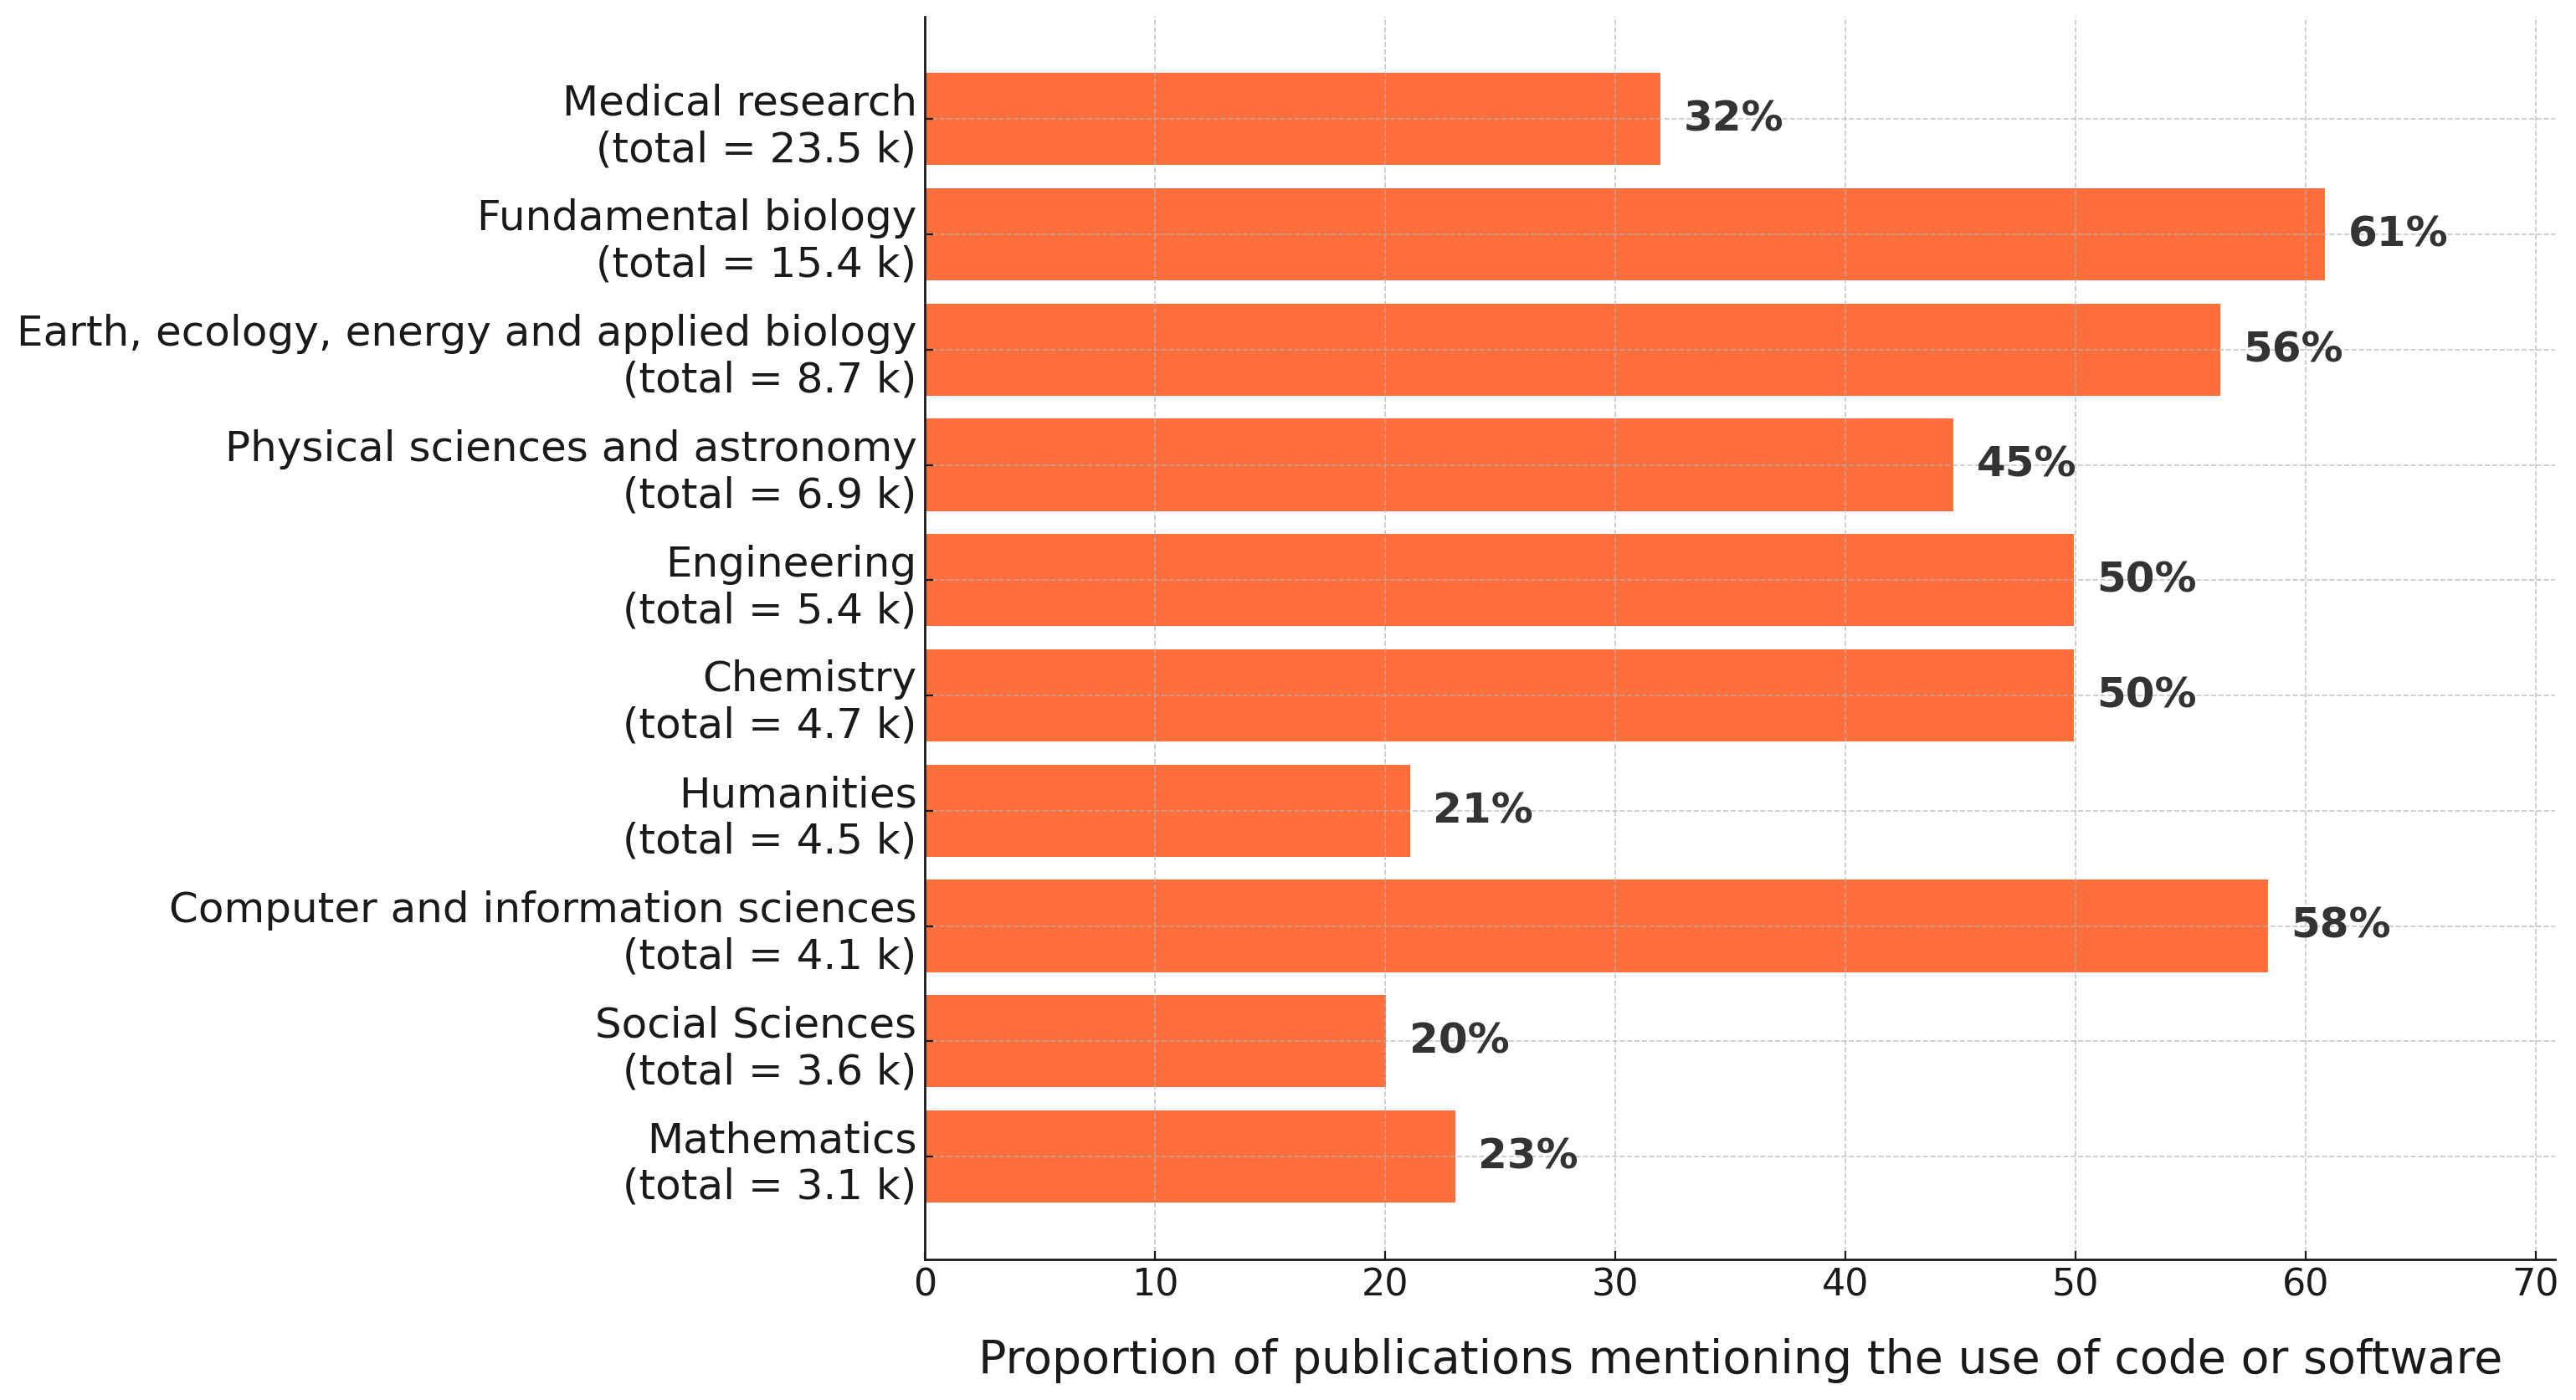
\includegraphics[width=\linewidth]{figures/french_os_monitor-use-2025.png}
  \caption[Software across all disciplines]{Across every discipline, a substantial and growing
  share of research articles produces or uses software. \emph{Source:} French Open Science
  Monitor, 2025 edition.}
  \label{fig:os-monitor}
\end{figure}

What makes software special is also what makes it easy to mishandle: it is at once executable
and human-readable; it \emph{evolves}, often over decades, so that its development history is
part of its meaning; and it never stands alone, resting instead on a deep web of other software
it depends on (Figure~\ref{fig:matplotlib-deps}). These are not the properties of a dataset ---
and, as we will see in the next
chapter, they are exactly the properties that the familiar, data-shaped recipes fail to
respect. Software is not data; it is a first-class citizen of the scientific record, and it
deserves to be treated as one.

\begin{figure}[htbp]
  \centering
  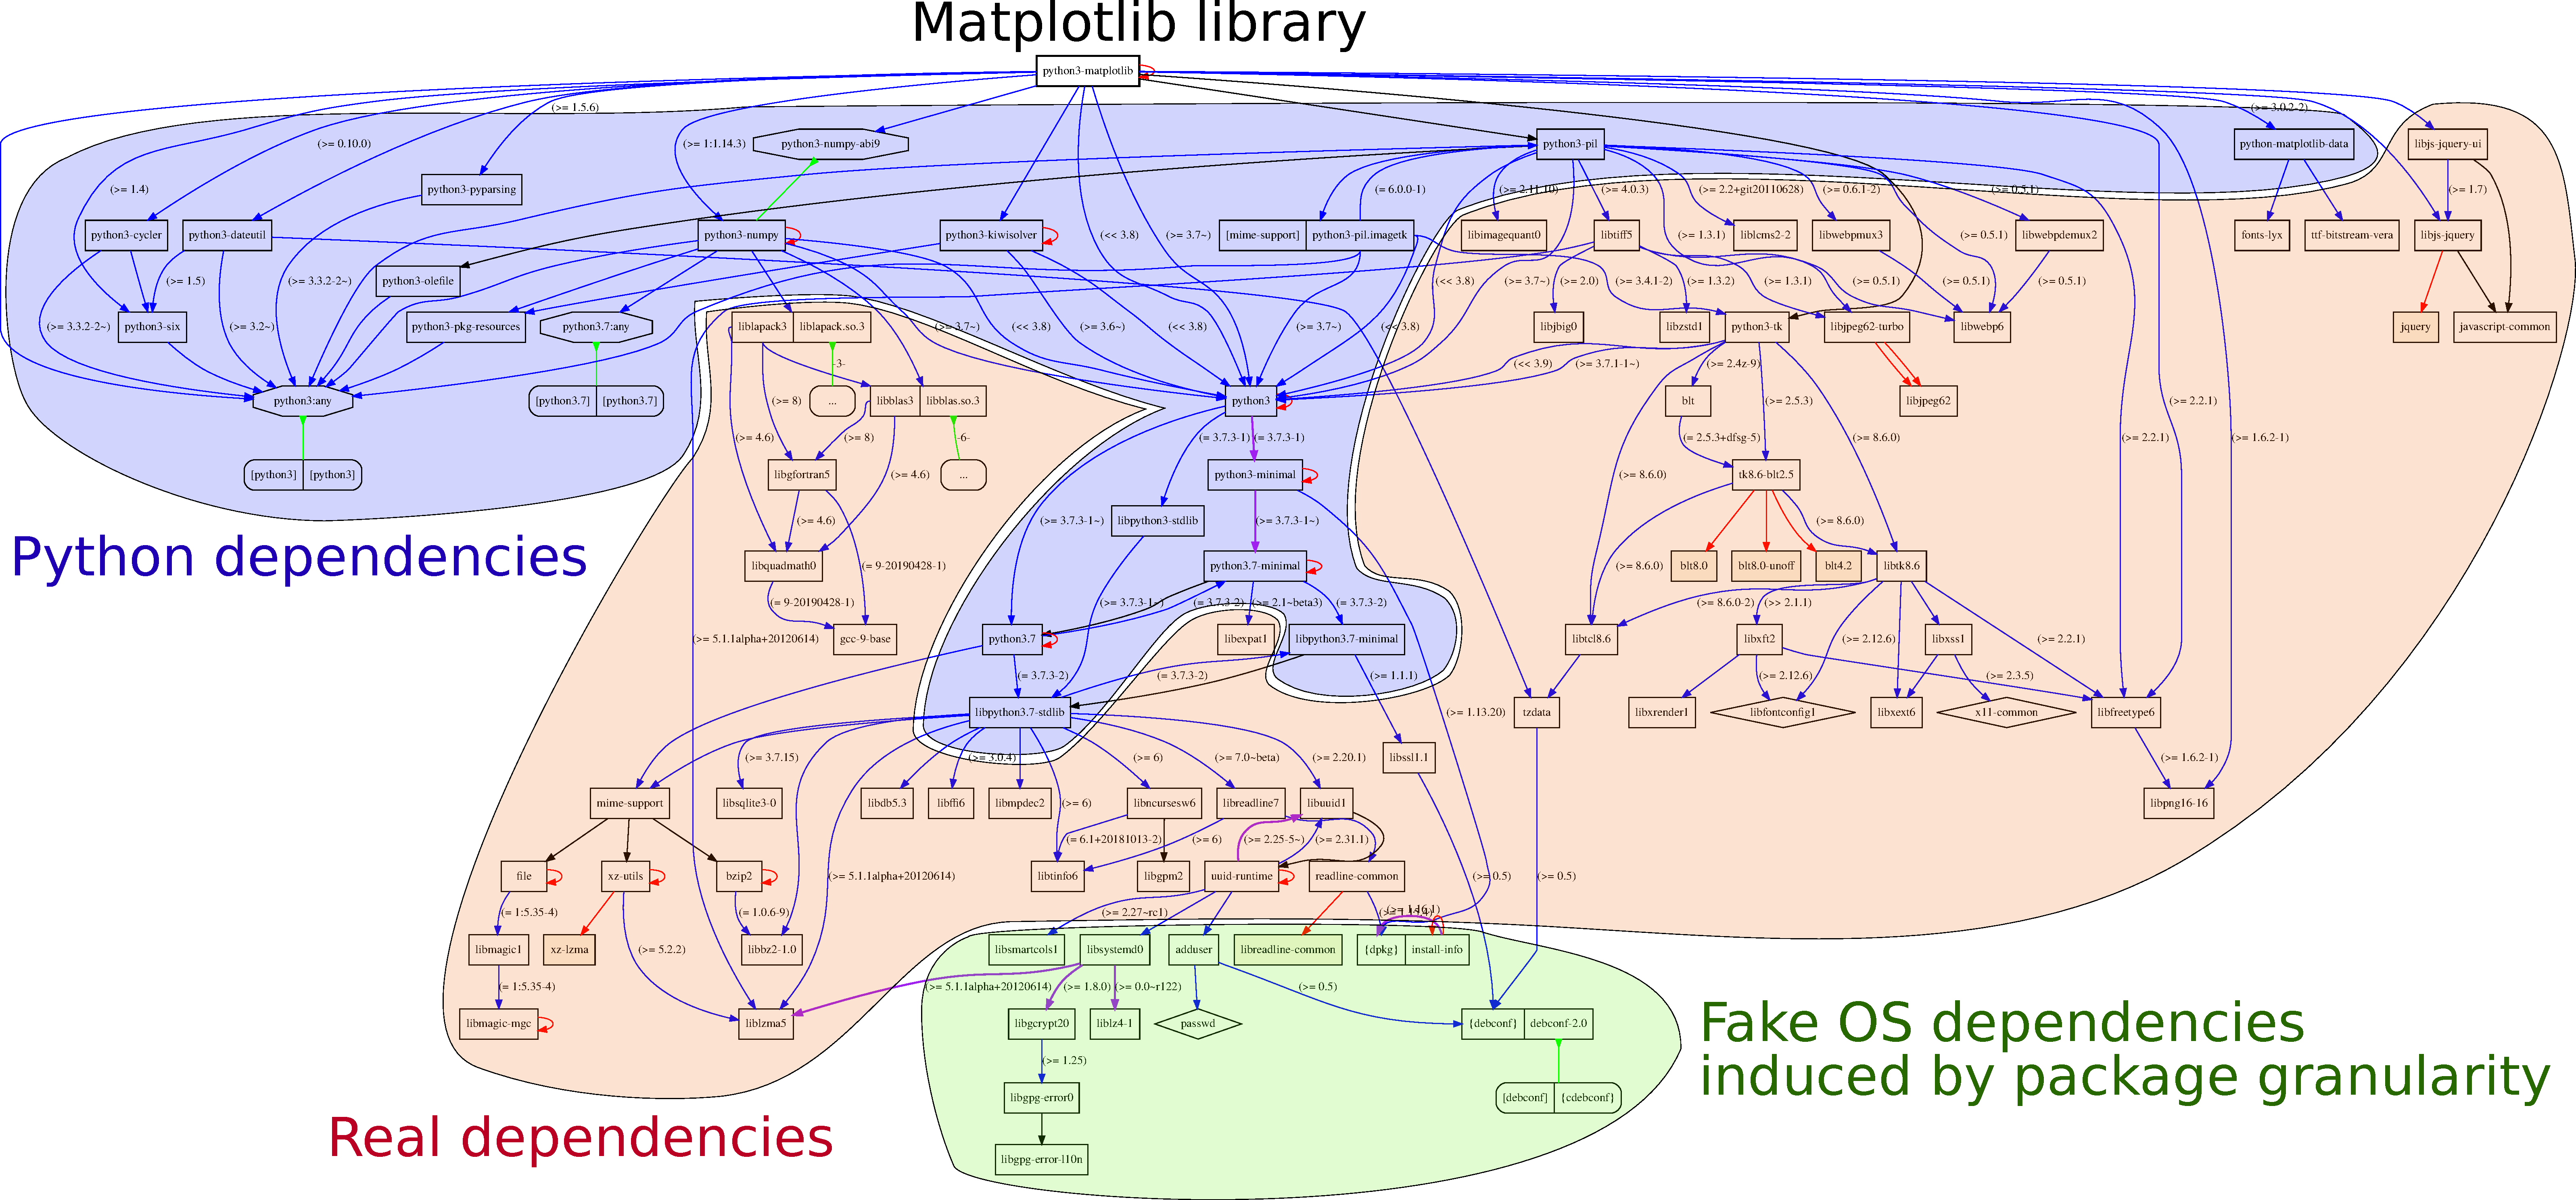
\includegraphics[width=\linewidth]{figures/python3-matplotlib.pdf}
  \caption[The dependency web of a single library]{No software stands alone. The dependency
  graph of the \texttt{matplotlib} plotting library: blue marks its Python-level dependencies,
  orange the real system libraries beneath, green the artefacts of packaging
  granularity~\autocite{SWHecosystems2023}. The individual labels are not meant to be read; the
  point is the \emph{density} --- a single research tool already rests on a deep web of other
  software, none of which the data-deposit model knows how to keep.}
  \label{fig:matplotlib-deps}
\end{figure}

\section{What is at stake}

The two most visible stakes are worth naming plainly, first.

The first is \emph{reproducibility}. A computational result is only as solid as our ability to
get hold of the exact code that produced it and run it again --- not code \emph{like} it, not a
later version with the bug quietly fixed, but \emph{that} code, at \emph{that} revision. We will
return to the dispiriting state of the art in Chapter~\ref{ch:repro}; for now it is enough to
say that, far too often, the code behind a published figure cannot be found, cannot be built, or
cannot be told apart from a dozen neighbouring versions.

The second is \emph{preservation}, and here a single slogan does most of the work: \emph{forges
are not archives}. GitHub, GitLab, and their kin are wonderful places to \emph{develop}
software; they make no promise whatsoever to \emph{keep} it. That promise has been tested, and
broken, more than once: Google Code and Gitorious shut down in 2015, putting roughly a million
repositories at risk; Bitbucket deleted more than 250,000 Mercurial repositories in 2020. The
half-life of a URL cited in the scholarly literature is about four years. Every one of those
losses is a hole in the web of knowledge --- a paper that points at code which is no longer
there.

\takeaway{Forges are for developing code; they make no promise to keep it.}

But reproducibility and preservation are only the most visible of a \emph{plurality} of needs ---
and those needs stack, scale by scale, each resting on the one beneath it.

A \emph{researcher} needs to archive and reference the exact code behind each result, so it can be
retrieved and re-run; to find and reuse the software of others; and --- not least --- to get
\emph{credit} for the software they build themselves, as for any other research output.

A \emph{laboratory or team director} needs to know what the group actually produces: to track its
software contributions, fold them into activity reports and a public software page, and not lose
them when the student who wrote them moves on.

A \emph{research organization} --- a university president, a funding agency --- needs to know its
\emph{software assets} at all: for technology transfer, for honest impact metrics, for funding
strategy, and for the fair career evaluation of the people who write software.

And here is the point that organises this whole note. Every one of these needs, from the lone result
to the institutional dashboard, rests on the same minimal foundation --- four things you must be
able to do to a piece of software: \textbf{archive} it (so it can be retrieved), \textbf{reference}
it exactly (so it can be identified), \textbf{describe} it (so it can be discovered and reused), and
\textbf{cite} it (so its authors are credited). Those four verbs --- \textbf{A}rchive,
\textbf{R}eference, \textbf{D}escribe, \textbf{C}ite \& credit, or \textsc{ardc} --- are the floor
beneath all the layers. Get them right, and reproducibility, visibility, and assessment all become
\emph{possible}; skip them, and none of the higher needs can be met, however much metadata or policy
is piled on top.

\takeaway{From the lone result to the institutional dashboard, every need rests on one floor:
\textsc{ardc}.}

And yet, collectively, we have not been taking good care of this precious form of
knowledge~\autocite{SwhCACM2018}. Closing that gap is the whole purpose of these notes.

\section{How to read these notes}

The good news is that \textsc{ardc} is not aspirational: the practice exists, the tools are built,
and you can adopt them today. It rests on two foundations --- the Software Heritage archive, which
preserves the world's source code with its full development history, and the \textsc{swhid}, an
identifier computed \emph{from the code itself} (and now the international standard ISO/IEC~18670)
that lets you point at exactly the code you mean. Chapter~\ref{ch:ardc} makes each of the four verbs
hands-on. We will meet the FAIR principles along the way and then, deliberately, go \emph{beyond}
them, for the reasons the next chapter makes precise~\autocite{NatureSD2026}.

These notes are meant to be read \emph{and} done. The practical chapters end with \textbf{Hands-on}
boxes you run on a repository of your choice --- your own code, a library you depend on, a result
you want to cite. Margin notes flag the one idea worth carrying away from each section; each chapter
opens with its \textbf{learning objectives}; and any unfamiliar term --- \textsc{swhid}, snapshot,
forge, qualified identifier --- is defined in the Glossary (Appendix~\ref{app:glossary}). And these
notes practise what they preach: they are themselves archived in Software Heritage, and the Colophon
shows you how to recompute and verify their own identifier --- the entire workflow, applied to the
very document in your hands.

You do not need to be a computer scientist to use any of this. Different readers will want
different routes through it:

\begin{callout}{Reading paths}
\small Pick a row and follow it; the rest can wait. The chapters do build on one another --- the
\textsc{swhid} (4) rests on the data model (3), and the practical core (5) uses both --- so a skipped
chapter is there when you need it.
\smallskip

\centering
\renewcommand{\arraystretch}{1.25}
\begin{tabular}{@{}l*{7}{c}c@{}}
\toprule
\textbf{Reader} & \textbf{1} & \textbf{2} & \textbf{3} & \textbf{4} & \textbf{5} & \textbf{6} & \textbf{7} & \textbf{App.}\\
\midrule
Researcher                     & \pathcore & \pathskip & \pathskip & \pathskim & \pathcore & \pathskim & \pathskip & A\\
Developer / intern             & \pathskim & \pathskip & \pathskip & \pathskim & \pathcore & \pathskip & \pathskip & A\\
Reviewer / editor / AEC        & \pathcore & \pathskip & \pathskip & \pathcore & \pathskim & \pathcore & \pathskip & ---\\
Funder / policy maker          & \pathcore & \pathskip & \pathskip & \pathskip & \pathskip & \pathskip & \pathcore & E\\
Full course / student          & \pathcore & \pathcore & \pathcore & \pathcore & \pathcore & \pathcore & \pathcore & all\\
\bottomrule
\end{tabular}

\smallskip
{\footnotesize \pathcore~core \quad \pathskim~skim / optional \quad \pathskip~skip. \quad
\textbf{1}~Why \enspace \textbf{2}~Beyond FAIR \enspace \textbf{3}~Foundations \enspace
\textbf{4}~The \textsc{swhid} \enspace \textbf{5}~\textsc{ardc} \enspace
\textbf{6}~Reproducibility \enspace \textbf{7}~Policy.}
\end{callout}

If you write or run code for your research --- whether a few lines of analysis or a library
maintained for decades --- these notes are for you. The tools are ready; the habit is the only thing
missing. Let us build it, starting with your next paper.
